\documentclass[twoside]{book}

% Packages required by doxygen
\usepackage{fixltx2e}
\usepackage{calc}
\usepackage{doxygen}
\usepackage[export]{adjustbox} % also loads graphicx
\usepackage{graphicx}
\usepackage[utf8]{inputenc}
\usepackage{makeidx}
\usepackage{multicol}
\usepackage{multirow}
\PassOptionsToPackage{warn}{textcomp}
\usepackage{textcomp}
\usepackage[nointegrals]{wasysym}
\usepackage[table]{xcolor}

% Font selection
\usepackage[T1]{fontenc}
\usepackage[scaled=.90]{helvet}
\usepackage{courier}
\usepackage{amssymb}
\usepackage{sectsty}
\renewcommand{\familydefault}{\sfdefault}
\allsectionsfont{%
  \fontseries{bc}\selectfont%
  \color{darkgray}%
}
\renewcommand{\DoxyLabelFont}{%
  \fontseries{bc}\selectfont%
  \color{darkgray}%
}
\newcommand{\+}{\discretionary{\mbox{\scriptsize$\hookleftarrow$}}{}{}}

% Page & text layout
\usepackage{geometry}
\geometry{%
  a4paper,%
  top=2.5cm,%
  bottom=2.5cm,%
  left=2.5cm,%
  right=2.5cm%
}
\tolerance=750
\hfuzz=15pt
\hbadness=750
\setlength{\emergencystretch}{15pt}
\setlength{\parindent}{0cm}
\setlength{\parskip}{3ex plus 2ex minus 2ex}
\makeatletter
\renewcommand{\paragraph}{%
  \@startsection{paragraph}{4}{0ex}{-1.0ex}{1.0ex}{%
    \normalfont\normalsize\bfseries\SS@parafont%
  }%
}
\renewcommand{\subparagraph}{%
  \@startsection{subparagraph}{5}{0ex}{-1.0ex}{1.0ex}{%
    \normalfont\normalsize\bfseries\SS@subparafont%
  }%
}
\makeatother

% Headers & footers
\usepackage{fancyhdr}
\pagestyle{fancyplain}
\fancyhead[LE]{\fancyplain{}{\bfseries\thepage}}
\fancyhead[CE]{\fancyplain{}{}}
\fancyhead[RE]{\fancyplain{}{\bfseries\leftmark}}
\fancyhead[LO]{\fancyplain{}{\bfseries\rightmark}}
\fancyhead[CO]{\fancyplain{}{}}
\fancyhead[RO]{\fancyplain{}{\bfseries\thepage}}
\fancyfoot[LE]{\fancyplain{}{}}
\fancyfoot[CE]{\fancyplain{}{}}
\fancyfoot[RE]{\fancyplain{}{\bfseries\scriptsize Generated by Doxygen }}
\fancyfoot[LO]{\fancyplain{}{\bfseries\scriptsize Generated by Doxygen }}
\fancyfoot[CO]{\fancyplain{}{}}
\fancyfoot[RO]{\fancyplain{}{}}
\renewcommand{\footrulewidth}{0.4pt}
\renewcommand{\chaptermark}[1]{%
  \markboth{#1}{}%
}
\renewcommand{\sectionmark}[1]{%
  \markright{\thesection\ #1}%
}

% Indices & bibliography
\usepackage{natbib}
\usepackage[titles]{tocloft}
\setcounter{tocdepth}{3}
\setcounter{secnumdepth}{5}
\makeindex

% Hyperlinks (required, but should be loaded last)
\usepackage{ifpdf}
\ifpdf
  \usepackage[pdftex,pagebackref=true]{hyperref}
\else
  \usepackage[ps2pdf,pagebackref=true]{hyperref}
\fi
\hypersetup{%
  colorlinks=true,%
  linkcolor=blue,%
  citecolor=blue,%
  unicode%
}

% Custom commands
\newcommand{\clearemptydoublepage}{%
  \newpage{\pagestyle{empty}\cleardoublepage}%
}

\usepackage{caption}
\captionsetup{labelsep=space,justification=centering,font={bf},singlelinecheck=off,skip=4pt,position=top}

%===== C O N T E N T S =====

\begin{document}

% Titlepage & ToC
\hypersetup{pageanchor=false,
             bookmarksnumbered=true,
             pdfencoding=unicode
            }
\pagenumbering{roman}
\begin{titlepage}
\vspace*{7cm}
\begin{center}%
{\Large Ackerman P\+ID Controller \\[1ex]\large 1 }\\
\vspace*{1cm}
{\large Generated by Doxygen 1.8.11}\\
\end{center}
\end{titlepage}
\clearemptydoublepage
\tableofcontents
\clearemptydoublepage
\pagenumbering{arabic}
\hypersetup{pageanchor=true}

%--- Begin generated contents ---
\chapter{Hierarchical Index}
\section{Class Hierarchy}
This inheritance list is sorted roughly, but not completely, alphabetically\+:\begin{DoxyCompactList}
\item \contentsline{section}{ackerman\+\_\+sim}{\pageref{classackerman__sim}}{}
\item \contentsline{section}{pid}{\pageref{classpid}}{}
\begin{DoxyCompactList}
\item \contentsline{section}{ackerman\+\_\+controller}{\pageref{classackerman__controller}}{}
\end{DoxyCompactList}
\end{DoxyCompactList}

\chapter{Class Index}
\section{Class List}
Here are the classes, structs, unions and interfaces with brief descriptions\+:\begin{DoxyCompactList}
\item\contentsline{section}{\hyperlink{classackerman__controller}{ackerman\+\_\+controller} }{\pageref{classackerman__controller}}{}
\item\contentsline{section}{\hyperlink{classackerman__sim}{ackerman\+\_\+sim} }{\pageref{classackerman__sim}}{}
\item\contentsline{section}{\hyperlink{classpid}{pid} }{\pageref{classpid}}{}
\end{DoxyCompactList}

\chapter{File Index}
\section{File List}
Here is a list of all documented files with brief descriptions\+:\begin{DoxyCompactList}
\item\contentsline{section}{app/\hyperlink{ackerman__controller_8cpp}{ackerman\+\_\+controller.\+cpp} \\*Defines the function to calculate the Radius, wheel velocity and update the current heading.  \char`\"{}\+Copyright 2019 $<$\+Ashwin Varghese Kuruttukulam$>$
@\+Copyright \char`\"{}Copyright 2019 $<$\+Charan karthikeyan$>$=\char`\"{}\char`\"{}$>$ }{\pageref{ackerman__controller_8cpp}}{}
\item\contentsline{section}{app/\hyperlink{ackerman__sim_8cpp}{ackerman\+\_\+sim.\+cpp} \\*Declarations of the function to simulate the ackerman steering  \char`\"{}\+Copyright 2019 $<$\+Ashwin Varghese Kuruttukulam$>$
@\+Copyright \char`\"{}Copyright 2019 $<$\+Charan karthikeyan$>$=\char`\"{}\char`\"{}$>$ }{\pageref{ackerman__sim_8cpp}}{}
\item\contentsline{section}{app/\hyperlink{main_8cpp}{main.\+cpp} \\*Main program that runs the pid, ackerman controller and the ackerman simulation classes }{\pageref{main_8cpp}}{}
\item\contentsline{section}{app/\hyperlink{pid_8cpp}{pid.\+cpp} \\*Definition of the P\+ID class to calculate the feedback  \char`\"{}\+Copyright 2019 $<$\+Ashwin Varghese Kuruttukulam$>$
@\+Copyright \char`\"{}Copyright 2019 $<$\+Charan karthikeyan$>$=\char`\"{}\char`\"{}$>$ }{\pageref{pid_8cpp}}{}
\item\contentsline{section}{include/{\bfseries ackerman\+\_\+controller.\+hpp} }{\pageref{ackerman__controller_8hpp}}{}
\item\contentsline{section}{include/\hyperlink{ackerman__sim_8hpp}{ackerman\+\_\+sim.\+hpp} \\*Defines the function to simulate the ackerman steering  \char`\"{}\+Copyright 2019 $<$\+Ashwin Varghese Kuruttukulam$>$
@\+Copyright \char`\"{}Copyright 2019 $<$\+Charan karthikeyan$>$=\char`\"{}\char`\"{}$>$ }{\pageref{ackerman__sim_8hpp}}{}
\item\contentsline{section}{include/\hyperlink{pid_8hpp}{pid.\+hpp} \\*Defines a P\+ID Controller from the feedback/measured value and the setpoint. The output of the P\+ID is calculated as per the equation output = Kp$\ast$\+Error + Ki$\ast$\+Error\+Sum$\ast$dt + Kp$\ast$(Error-\/prev\+Error)/dt }{\pageref{pid_8hpp}}{}
\end{DoxyCompactList}

\chapter{Class Documentation}
\hypertarget{classackerman__controller}{}\section{ackerman\+\_\+controller Class Reference}
\label{classackerman__controller}\index{ackerman\+\_\+controller@{ackerman\+\_\+controller}}


Inheritance diagram for ackerman\+\_\+controller\+:
\nopagebreak
\begin{figure}[H]
\begin{center}
\leavevmode
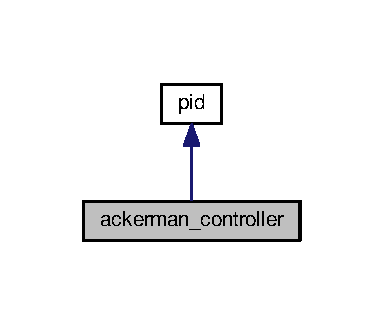
\includegraphics[width=184pt]{classackerman__controller__inherit__graph}
\end{center}
\end{figure}


Collaboration diagram for ackerman\+\_\+controller\+:
\nopagebreak
\begin{figure}[H]
\begin{center}
\leavevmode
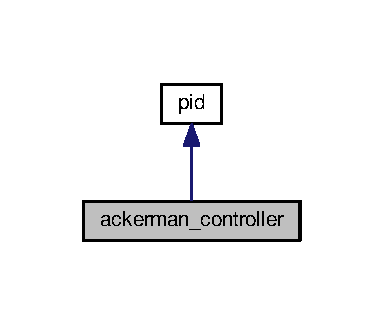
\includegraphics[width=184pt]{classackerman__controller__coll__graph}
\end{center}
\end{figure}
\subsection*{Public Member Functions}
\begin{DoxyCompactItemize}
\item 
\hyperlink{classackerman__controller_a2501aaf8866f31033b029135e9a07a06}{ackerman\+\_\+controller} (double baseline, double car\+Length)
\begin{DoxyCompactList}\small\item\em Initialize the car parameters. \end{DoxyCompactList}\item 
\hyperlink{classackerman__controller_a8ce4def42fb84ddd2d0ead34b99c0724}{ackerman\+\_\+controller} (double baseline, double car\+Len, double kp, double ki, double kd, bool dt\+Mode, double dt)
\begin{DoxyCompactList}\small\item\em Second Constructor to initialize all the parameters. \end{DoxyCompactList}\item 
double \hyperlink{classackerman__controller_a5638d86309c34d185bed37275c153c65}{get\+Heading\+Points} ()
\begin{DoxyCompactList}\small\item\em Function to get the value of the heading setpoints. \end{DoxyCompactList}\item 
double \hyperlink{classackerman__controller_aaf95cf16e95bce3a68625e7f7d57c45e}{get\+Velocity\+Points} ()
\begin{DoxyCompactList}\small\item\em Function to get the values of velocity setpoints. \end{DoxyCompactList}\item 
double \hyperlink{classackerman__controller_a2b08918e113a5ae0ebd1b976801bec7c}{run} (double heading\+Feedback, double \&r\+Wheel\+Vel, double \&l\+Wheel\+Vel)
\begin{DoxyCompactList}\small\item\em Function to compute the steering angle, wheel velocity of the right and left wheels. \end{DoxyCompactList}\item 
void \hyperlink{classackerman__controller_aba2b7c99bcdcd50e5ea36012fe849000}{set\+Set\+Points} (double headingsp, double velocitysp)
\begin{DoxyCompactList}\small\item\em Function to update the target points. \end{DoxyCompactList}\item 
double \hyperlink{classackerman__controller_a44b85e8dceca2ec8112c5bc87d16d319}{get\+Base\+Line} ()
\begin{DoxyCompactList}\small\item\em Function to get the value of baseline (for testing purpose only) \end{DoxyCompactList}\item 
double \hyperlink{classackerman__controller_a206a0b3afc07d1f12769f2a75515c7e8}{get\+Car\+Len} ()
\begin{DoxyCompactList}\small\item\em Function to return the value of car length (For testing purpose only) \end{DoxyCompactList}\end{DoxyCompactItemize}


\subsection{Constructor \& Destructor Documentation}
\index{ackerman\+\_\+controller@{ackerman\+\_\+controller}!ackerman\+\_\+controller@{ackerman\+\_\+controller}}
\index{ackerman\+\_\+controller@{ackerman\+\_\+controller}!ackerman\+\_\+controller@{ackerman\+\_\+controller}}
\subsubsection[{\texorpdfstring{ackerman\+\_\+controller(double baseline, double car\+Length)}{ackerman_controller(double baseline, double carLength)}}]{\setlength{\rightskip}{0pt plus 5cm}ackerman\+\_\+controller\+::ackerman\+\_\+controller (
\begin{DoxyParamCaption}
\item[{double}]{baseline, }
\item[{double}]{car\+Length}
\end{DoxyParamCaption}
)}\hypertarget{classackerman__controller_a2501aaf8866f31033b029135e9a07a06}{}\label{classackerman__controller_a2501aaf8866f31033b029135e9a07a06}


Initialize the car parameters. 


\begin{DoxyParams}{Parameters}
{\em distance} & between left and right wheels(baseline) \\
\hline
{\em distance} & between front and back wheels(car\+Length) \\
\hline
\end{DoxyParams}
\begin{DoxyReturn}{Returns}

\end{DoxyReturn}
\index{ackerman\+\_\+controller@{ackerman\+\_\+controller}!ackerman\+\_\+controller@{ackerman\+\_\+controller}}
\index{ackerman\+\_\+controller@{ackerman\+\_\+controller}!ackerman\+\_\+controller@{ackerman\+\_\+controller}}
\subsubsection[{\texorpdfstring{ackerman\+\_\+controller(double baseline, double car\+Len, double kp, double ki, double kd, bool dt\+Mode, double dt)}{ackerman_controller(double baseline, double carLen, double kp, double ki, double kd, bool dtMode, double dt)}}]{\setlength{\rightskip}{0pt plus 5cm}ackerman\+\_\+controller\+::ackerman\+\_\+controller (
\begin{DoxyParamCaption}
\item[{double}]{baseline, }
\item[{double}]{car\+Len, }
\item[{double}]{kp, }
\item[{double}]{ki, }
\item[{double}]{kd, }
\item[{bool}]{dt\+Mode, }
\item[{double}]{dt}
\end{DoxyParamCaption}
)}\hypertarget{classackerman__controller_a8ce4def42fb84ddd2d0ead34b99c0724}{}\label{classackerman__controller_a8ce4def42fb84ddd2d0ead34b99c0724}


Second Constructor to initialize all the parameters. 


\begin{DoxyParams}{Parameters}
{\em The} & distance between the two wheels of a car(baseline) \\
\hline
{\em The} & distance between the front and back of the vehicle(car\+Len) \\
\hline
{\em The} & integral gain(ki) \\
\hline
{\em The} & Propotional gain(kp) \\
\hline
{\em The} & differential gain(kd) \\
\hline
{\em The} & mode of operation for the \hyperlink{classpid}{pid(dt\+Mode)} true for automatic and false for manual. \\
\hline
{\em The} & change in time (dt) \\
\hline
\end{DoxyParams}
\begin{DoxyReturn}{Returns}
None. 
\end{DoxyReturn}


\subsection{Member Function Documentation}
\index{ackerman\+\_\+controller@{ackerman\+\_\+controller}!get\+Base\+Line@{get\+Base\+Line}}
\index{get\+Base\+Line@{get\+Base\+Line}!ackerman\+\_\+controller@{ackerman\+\_\+controller}}
\subsubsection[{\texorpdfstring{get\+Base\+Line()}{getBaseLine()}}]{\setlength{\rightskip}{0pt plus 5cm}double ackerman\+\_\+controller\+::get\+Base\+Line (
\begin{DoxyParamCaption}
{}
\end{DoxyParamCaption}
)}\hypertarget{classackerman__controller_a44b85e8dceca2ec8112c5bc87d16d319}{}\label{classackerman__controller_a44b85e8dceca2ec8112c5bc87d16d319}


Function to get the value of baseline (for testing purpose only) 


\begin{DoxyParams}{Parameters}
{\em None} & \\
\hline
\end{DoxyParams}
\begin{DoxyReturn}{Returns}
The value baseline 
\end{DoxyReturn}
\index{ackerman\+\_\+controller@{ackerman\+\_\+controller}!get\+Car\+Len@{get\+Car\+Len}}
\index{get\+Car\+Len@{get\+Car\+Len}!ackerman\+\_\+controller@{ackerman\+\_\+controller}}
\subsubsection[{\texorpdfstring{get\+Car\+Len()}{getCarLen()}}]{\setlength{\rightskip}{0pt plus 5cm}double ackerman\+\_\+controller\+::get\+Car\+Len (
\begin{DoxyParamCaption}
{}
\end{DoxyParamCaption}
)}\hypertarget{classackerman__controller_a206a0b3afc07d1f12769f2a75515c7e8}{}\label{classackerman__controller_a206a0b3afc07d1f12769f2a75515c7e8}


Function to return the value of car length (For testing purpose only) 


\begin{DoxyParams}{Parameters}
{\em None.} & \\
\hline
\end{DoxyParams}
\begin{DoxyReturn}{Returns}
The value of the length of the car 
\end{DoxyReturn}
\index{ackerman\+\_\+controller@{ackerman\+\_\+controller}!get\+Heading\+Points@{get\+Heading\+Points}}
\index{get\+Heading\+Points@{get\+Heading\+Points}!ackerman\+\_\+controller@{ackerman\+\_\+controller}}
\subsubsection[{\texorpdfstring{get\+Heading\+Points()}{getHeadingPoints()}}]{\setlength{\rightskip}{0pt plus 5cm}double ackerman\+\_\+controller\+::get\+Heading\+Points (
\begin{DoxyParamCaption}
{}
\end{DoxyParamCaption}
)}\hypertarget{classackerman__controller_a5638d86309c34d185bed37275c153c65}{}\label{classackerman__controller_a5638d86309c34d185bed37275c153c65}


Function to get the value of the heading setpoints. 


\begin{DoxyParams}{Parameters}
{\em None.} & \\
\hline
\end{DoxyParams}
\begin{DoxyReturn}{Returns}
Points of the heading. 
\end{DoxyReturn}
\index{ackerman\+\_\+controller@{ackerman\+\_\+controller}!get\+Velocity\+Points@{get\+Velocity\+Points}}
\index{get\+Velocity\+Points@{get\+Velocity\+Points}!ackerman\+\_\+controller@{ackerman\+\_\+controller}}
\subsubsection[{\texorpdfstring{get\+Velocity\+Points()}{getVelocityPoints()}}]{\setlength{\rightskip}{0pt plus 5cm}double ackerman\+\_\+controller\+::get\+Velocity\+Points (
\begin{DoxyParamCaption}
{}
\end{DoxyParamCaption}
)}\hypertarget{classackerman__controller_aaf95cf16e95bce3a68625e7f7d57c45e}{}\label{classackerman__controller_aaf95cf16e95bce3a68625e7f7d57c45e}


Function to get the values of velocity setpoints. 


\begin{DoxyParams}{Parameters}
{\em None.} & \\
\hline
\end{DoxyParams}
\begin{DoxyReturn}{Returns}
Points for the Velocity points. 
\end{DoxyReturn}
\index{ackerman\+\_\+controller@{ackerman\+\_\+controller}!run@{run}}
\index{run@{run}!ackerman\+\_\+controller@{ackerman\+\_\+controller}}
\subsubsection[{\texorpdfstring{run(double heading\+Feedback, double \&r\+Wheel\+Vel, double \&l\+Wheel\+Vel)}{run(double headingFeedback, double &rWheelVel, double &lWheelVel)}}]{\setlength{\rightskip}{0pt plus 5cm}double ackerman\+\_\+controller\+::run (
\begin{DoxyParamCaption}
\item[{double}]{heading\+Feedback, }
\item[{double \&}]{r\+Wheel\+Vel, }
\item[{double \&}]{l\+Wheel\+Vel}
\end{DoxyParamCaption}
)}\hypertarget{classackerman__controller_a2b08918e113a5ae0ebd1b976801bec7c}{}\label{classackerman__controller_a2b08918e113a5ae0ebd1b976801bec7c}


Function to compute the steering angle, wheel velocity of the right and left wheels. 


\begin{DoxyParams}{Parameters}
{\em The} & feedback about the heading from the P\+ID controller(heading\+Feedback). \\
\hline
{\em The} & velocity of the right and left wheels(r\+Wheel\+Vel, l\+Wheel\+Vel)(only for testing we use these values) \\
\hline
\end{DoxyParams}
\begin{DoxyReturn}{Returns}
The values of steering angle, the velocity of the right and left wheels. 
\end{DoxyReturn}
\index{ackerman\+\_\+controller@{ackerman\+\_\+controller}!set\+Set\+Points@{set\+Set\+Points}}
\index{set\+Set\+Points@{set\+Set\+Points}!ackerman\+\_\+controller@{ackerman\+\_\+controller}}
\subsubsection[{\texorpdfstring{set\+Set\+Points(double headingsp, double velocitysp)}{setSetPoints(double headingsp, double velocitysp)}}]{\setlength{\rightskip}{0pt plus 5cm}void ackerman\+\_\+controller\+::set\+Set\+Points (
\begin{DoxyParamCaption}
\item[{double}]{headingsp, }
\item[{double}]{velocitysp}
\end{DoxyParamCaption}
)}\hypertarget{classackerman__controller_aba2b7c99bcdcd50e5ea36012fe849000}{}\label{classackerman__controller_aba2b7c99bcdcd50e5ea36012fe849000}


Function to update the target points. 


\begin{DoxyParams}{Parameters}
{\em heading} & set point of the target point(headingsp) \\
\hline
{\em velocity} & of the set point(velocitysp) \\
\hline
\end{DoxyParams}
\begin{DoxyReturn}{Returns}
None. 
\end{DoxyReturn}


The documentation for this class was generated from the following files\+:\begin{DoxyCompactItemize}
\item 
include/ackerman\+\_\+controller.\+hpp\item 
app/\hyperlink{ackerman__controller_8cpp}{ackerman\+\_\+controller.\+cpp}\end{DoxyCompactItemize}

\hypertarget{classackerman__sim}{}\section{ackerman\+\_\+sim Class Reference}
\label{classackerman__sim}\index{ackerman\+\_\+sim@{ackerman\+\_\+sim}}
\subsection*{Public Member Functions}
\begin{DoxyCompactItemize}
\item 
\hyperlink{classackerman__sim_adc6ee573b9cfc562f439ee0d9ad75121}{ackerman\+\_\+sim} ()
\begin{DoxyCompactList}\small\item\em A Constructor for the simulator. \end{DoxyCompactList}\item 
\hyperlink{classackerman__sim_a74a90d213df76c3fe4f8c1f29fa3b668}{ackerman\+\_\+sim} (double dt)
\begin{DoxyCompactList}\small\item\em A constructor for the ackerman simulation. \end{DoxyCompactList}\item 
\hyperlink{classackerman__sim_a142ee1c5be5f84b1ba94091be817ce65}{$\sim$ackerman\+\_\+sim} ()
\begin{DoxyCompactList}\small\item\em Destructor for the ackerman simulation. \end{DoxyCompactList}\item 
void \hyperlink{classackerman__sim_a942b5493103ae31ab1a0c6868a0f2de8}{compute} (double steer\+Ang, double r\+Wheel\+Vel, double l\+Wheel\+Vel, double \&posX, double \&posY, double \&updated\+Heading, double car\+Len)
\begin{DoxyCompactList}\small\item\em This function is called to update the vehicle heading as per the wheel velocities and the steering angle. \end{DoxyCompactList}\end{DoxyCompactItemize}


\subsection{Constructor \& Destructor Documentation}
\index{ackerman\+\_\+sim@{ackerman\+\_\+sim}!ackerman\+\_\+sim@{ackerman\+\_\+sim}}
\index{ackerman\+\_\+sim@{ackerman\+\_\+sim}!ackerman\+\_\+sim@{ackerman\+\_\+sim}}
\subsubsection[{\texorpdfstring{ackerman\+\_\+sim()}{ackerman_sim()}}]{\setlength{\rightskip}{0pt plus 5cm}ackerman\+\_\+sim\+::ackerman\+\_\+sim (
\begin{DoxyParamCaption}
{}
\end{DoxyParamCaption}
)}\hypertarget{classackerman__sim_adc6ee573b9cfc562f439ee0d9ad75121}{}\label{classackerman__sim_adc6ee573b9cfc562f439ee0d9ad75121}


A Constructor for the simulator. 


\begin{DoxyParams}{Parameters}
{\em None.} & \\
\hline
\end{DoxyParams}
\begin{DoxyReturn}{Returns}
None. 
\end{DoxyReturn}
\index{ackerman\+\_\+sim@{ackerman\+\_\+sim}!ackerman\+\_\+sim@{ackerman\+\_\+sim}}
\index{ackerman\+\_\+sim@{ackerman\+\_\+sim}!ackerman\+\_\+sim@{ackerman\+\_\+sim}}
\subsubsection[{\texorpdfstring{ackerman\+\_\+sim(double dt)}{ackerman_sim(double dt)}}]{\setlength{\rightskip}{0pt plus 5cm}ackerman\+\_\+sim\+::ackerman\+\_\+sim (
\begin{DoxyParamCaption}
\item[{double}]{dt}
\end{DoxyParamCaption}
)}\hypertarget{classackerman__sim_a74a90d213df76c3fe4f8c1f29fa3b668}{}\label{classackerman__sim_a74a90d213df76c3fe4f8c1f29fa3b668}


A constructor for the ackerman simulation. 


\begin{DoxyParams}{Parameters}
{\em Change} & in time(dt) \\
\hline
\end{DoxyParams}
\begin{DoxyReturn}{Returns}
None. 
\end{DoxyReturn}
\index{ackerman\+\_\+sim@{ackerman\+\_\+sim}!````~ackerman\+\_\+sim@{$\sim$ackerman\+\_\+sim}}
\index{````~ackerman\+\_\+sim@{$\sim$ackerman\+\_\+sim}!ackerman\+\_\+sim@{ackerman\+\_\+sim}}
\subsubsection[{\texorpdfstring{$\sim$ackerman\+\_\+sim()}{~ackerman_sim()}}]{\setlength{\rightskip}{0pt plus 5cm}ackerman\+\_\+sim\+::$\sim$ackerman\+\_\+sim (
\begin{DoxyParamCaption}
{}
\end{DoxyParamCaption}
)}\hypertarget{classackerman__sim_a142ee1c5be5f84b1ba94091be817ce65}{}\label{classackerman__sim_a142ee1c5be5f84b1ba94091be817ce65}


Destructor for the ackerman simulation. 


\begin{DoxyParams}{Parameters}
{\em None.} & return None. \\
\hline
\end{DoxyParams}


\subsection{Member Function Documentation}
\index{ackerman\+\_\+sim@{ackerman\+\_\+sim}!compute@{compute}}
\index{compute@{compute}!ackerman\+\_\+sim@{ackerman\+\_\+sim}}
\subsubsection[{\texorpdfstring{compute(double steer\+Ang, double r\+Wheel\+Vel, double l\+Wheel\+Vel, double \&pos\+X, double \&pos\+Y, double \&updated\+Heading, double car\+Len)}{compute(double steerAng, double rWheelVel, double lWheelVel, double &posX, double &posY, double &updatedHeading, double carLen)}}]{\setlength{\rightskip}{0pt plus 5cm}void ackerman\+\_\+sim\+::compute (
\begin{DoxyParamCaption}
\item[{double}]{steer\+Ang, }
\item[{double}]{r\+Wheel\+Vel, }
\item[{double}]{l\+Wheel\+Vel, }
\item[{double \&}]{posX, }
\item[{double \&}]{posY, }
\item[{double \&}]{updated\+Heading, }
\item[{double}]{car\+Len}
\end{DoxyParamCaption}
)}\hypertarget{classackerman__sim_a942b5493103ae31ab1a0c6868a0f2de8}{}\label{classackerman__sim_a942b5493103ae31ab1a0c6868a0f2de8}


This function is called to update the vehicle heading as per the wheel velocities and the steering angle. 


\begin{DoxyParams}{Parameters}
{\em The} & steering angle computed for the car(steer\+Ang) \\
\hline
{\em The} & velocity of the right wheel(r\+Wheel\+Vel) \\
\hline
{\em The} & velocity of the left wheel(l\+Wheel\+Vel) \\
\hline
{\em The} & positionf the vehicle in the x axis(posx) \\
\hline
{\em The} & positionf the vehicle in the y axis(posy) \\
\hline
{\em The} & length of the car or vehiclr(car\+Len) \\
\hline
{\em The} & updated heading of the vehicle(updated\+Heading) \\
\hline
\end{DoxyParams}
\begin{DoxyReturn}{Returns}
The x position, y position and new heading 
\end{DoxyReturn}


The documentation for this class was generated from the following files\+:\begin{DoxyCompactItemize}
\item 
include/\hyperlink{ackerman__sim_8hpp}{ackerman\+\_\+sim.\+hpp}\item 
app/\hyperlink{ackerman__sim_8cpp}{ackerman\+\_\+sim.\+cpp}\end{DoxyCompactItemize}

\hypertarget{classpid}{}\section{pid Class Reference}
\label{classpid}\index{pid@{pid}}


Inheritance diagram for pid\+:
\nopagebreak
\begin{figure}[H]
\begin{center}
\leavevmode
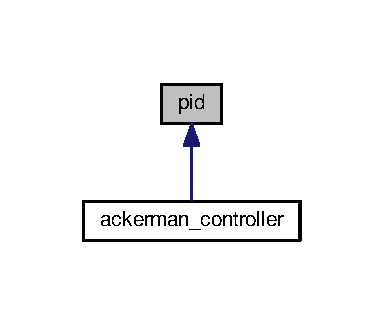
\includegraphics[width=184pt]{classpid__inherit__graph}
\end{center}
\end{figure}
\subsection*{Public Member Functions}
\begin{DoxyCompactItemize}
\item 
\hyperlink{classpid_a8cb9ff8fa0e7162d275990d01fb1588d}{pid} ()
\begin{DoxyCompactList}\small\item\em Constructor for the P\+ID Controller, Initialize kp to 1, ki and kd to 0. \end{DoxyCompactList}\item 
\hyperlink{classpid_aca31b4446bc7cafef37bf0ed799433c5}{pid} (double kp, double ki, double kd)
\begin{DoxyCompactList}\small\item\em Initialize the pid gain parameters to the parameter values. \end{DoxyCompactList}\item 
\hyperlink{classpid_afa844eff521e7d10d13008bb1befe6fe}{pid} (double kp, double ki, double kd, bool dt\+Mode)
\begin{DoxyCompactList}\small\item\em Initialize the pid gain parameters to the parameter values and set the dt mode type dt\+Mode = true means that the user will set the dt value and ensure that the compute function is called at every dt seconds. \end{DoxyCompactList}\item 
double \hyperlink{classpid_a3cd146c6f8b82f884106d1686b74f095}{compute} (double feedback)
\begin{DoxyCompactList}\small\item\em Destructor for the P\+ID Controller. \end{DoxyCompactList}\item 
void \hyperlink{classpid_ad79422e5b67012c47eb967606343df35}{setdt\+Mode} (bool dt\+Mode)
\begin{DoxyCompactList}\small\item\em Function to set the value of bool to trigger automatic or manual setting of dt of the P\+ID controller. \end{DoxyCompactList}\item 
void \hyperlink{classpid_a6c035fb6eaa1ec6a4113c318571bfd8b}{setdt} (double dt)
\begin{DoxyCompactList}\small\item\em Function to set the value of the change in time value. \end{DoxyCompactList}\item 
void \hyperlink{classpid_a08673f8deebcfd4ff97c7794739a1a5a}{set\+Sp} (double set\+Point)
\begin{DoxyCompactList}\small\item\em Function to set the value of set\+Point for the target heading. \end{DoxyCompactList}\item 
void \hyperlink{classpid_a4ceef80aa2e2e6dc49eead967c288f26}{setkp} (double)
\begin{DoxyCompactList}\small\item\em Function to set the value of Proportional Gain of the P\+ID controller. \end{DoxyCompactList}\item 
void \hyperlink{classpid_a98faeb432f25a5729fc8a48ade1ed6de}{setki} (double)
\begin{DoxyCompactList}\small\item\em Function to set the value of Integral Gain of the P\+ID controller. \end{DoxyCompactList}\item 
void \hyperlink{classpid_ae062827b4cb59a99e941d23cca3eb677}{setkd} (double)
\begin{DoxyCompactList}\small\item\em Function to set the value for Differential Gain of the P\+ID controller. \end{DoxyCompactList}\item 
bool \hyperlink{classpid_a2c94e73a942950ebefe98863bb391cbf}{getdt\+Mode} ()
\begin{DoxyCompactList}\small\item\em returns the value of boolean of the change in time mode for the controller \end{DoxyCompactList}\item 
double \hyperlink{classpid_a9b541ca0e6644a20c89d4c84922cf63a}{getdt} ()
\begin{DoxyCompactList}\small\item\em returns the value of the change in time set. \end{DoxyCompactList}\item 
double \hyperlink{classpid_a7c38309ebf1be92157ca45103ca15c6a}{get\+Sp} ()
\begin{DoxyCompactList}\small\item\em returns the value of set\+Point for the target heading \end{DoxyCompactList}\item 
double \hyperlink{classpid_a019f96dceec59007fa9823f56e8e9dd1}{getkp} ()
\begin{DoxyCompactList}\small\item\em Function to get the value of Proportional Gain of the P\+ID controller. \end{DoxyCompactList}\item 
double \hyperlink{classpid_a55be3ce4dfbf2527c92a05e2e6fdeb99}{getki} ()
\begin{DoxyCompactList}\small\item\em returns the value of the Integral Gain of the P\+ID controller \end{DoxyCompactList}\item 
double \hyperlink{classpid_aa1e0dfeb8630d336d00effeb2821a44e}{get\+Error\+Sum} ()
\begin{DoxyCompactList}\small\item\em Function to return the value of the error sum and test purposes. \end{DoxyCompactList}\item 
double \hyperlink{classpid_a5a03d1dffdb5b46d8b069a7a15aba033}{getkd} ()
\begin{DoxyCompactList}\small\item\em returns the value of the Differential Gain of the P\+ID controller \end{DoxyCompactList}\item 
double \hyperlink{classpid_a2ecb768afc444a7d65a56ae5d386d15e}{get\+Prev\+Error} ()
\begin{DoxyCompactList}\small\item\em Function to return the value of previous error for testing purposes. \end{DoxyCompactList}\item 
void \hyperlink{classpid_a06e0eda908ef2c8904135caeb56fd3e0}{reset} ()
\begin{DoxyCompactList}\small\item\em Function to reset the integral term to zero. \end{DoxyCompactList}\end{DoxyCompactItemize}


\subsection{Constructor \& Destructor Documentation}
\index{pid@{pid}!pid@{pid}}
\index{pid@{pid}!pid@{pid}}
\subsubsection[{\texorpdfstring{pid()}{pid()}}]{\setlength{\rightskip}{0pt plus 5cm}pid\+::pid (
\begin{DoxyParamCaption}
{}
\end{DoxyParamCaption}
)}\hypertarget{classpid_a8cb9ff8fa0e7162d275990d01fb1588d}{}\label{classpid_a8cb9ff8fa0e7162d275990d01fb1588d}


Constructor for the P\+ID Controller, Initialize kp to 1, ki and kd to 0. 


\begin{DoxyParams}{Parameters}
{\em None.} & \\
\hline
\end{DoxyParams}
\begin{DoxyReturn}{Returns}
None. 
\end{DoxyReturn}
\index{pid@{pid}!pid@{pid}}
\index{pid@{pid}!pid@{pid}}
\subsubsection[{\texorpdfstring{pid(double kp, double ki, double kd)}{pid(double kp, double ki, double kd)}}]{\setlength{\rightskip}{0pt plus 5cm}pid\+::pid (
\begin{DoxyParamCaption}
\item[{double}]{kp, }
\item[{double}]{ki, }
\item[{double}]{kd}
\end{DoxyParamCaption}
)}\hypertarget{classpid_aca31b4446bc7cafef37bf0ed799433c5}{}\label{classpid_aca31b4446bc7cafef37bf0ed799433c5}


Initialize the pid gain parameters to the parameter values. 


\begin{DoxyParams}{Parameters}
{\em kp} & Proportional Gain of P\+ID controller. \\
\hline
{\em ki} & Integral Gain of P\+ID controller. \\
\hline
{\em kd} & Differential Gain of P\+ID controller. \\
\hline
\end{DoxyParams}
\begin{DoxyReturn}{Returns}
None. 
\end{DoxyReturn}
\index{pid@{pid}!pid@{pid}}
\index{pid@{pid}!pid@{pid}}
\subsubsection[{\texorpdfstring{pid(double kp, double ki, double kd, bool dt\+Mode)}{pid(double kp, double ki, double kd, bool dtMode)}}]{\setlength{\rightskip}{0pt plus 5cm}pid\+::pid (
\begin{DoxyParamCaption}
\item[{double}]{kp, }
\item[{double}]{ki, }
\item[{double}]{kd, }
\item[{bool}]{dt\+Mode}
\end{DoxyParamCaption}
)}\hypertarget{classpid_afa844eff521e7d10d13008bb1befe6fe}{}\label{classpid_afa844eff521e7d10d13008bb1befe6fe}


Initialize the pid gain parameters to the parameter values and set the dt mode type dt\+Mode = true means that the user will set the dt value and ensure that the compute function is called at every dt seconds. 


\begin{DoxyParams}{Parameters}
{\em kp} & Proportional Gain of P\+ID controller. \\
\hline
{\em ki} & Integral Gain of P\+ID controller. \\
\hline
{\em kd} & Differential Gain of P\+ID controller. \\
\hline
{\em dt\+Mode} & Mode in which the pid controller works. \\
\hline
\end{DoxyParams}
\begin{DoxyReturn}{Returns}
None. 
\end{DoxyReturn}


\subsection{Member Function Documentation}
\index{pid@{pid}!compute@{compute}}
\index{compute@{compute}!pid@{pid}}
\subsubsection[{\texorpdfstring{compute(double feedback)}{compute(double feedback)}}]{\setlength{\rightskip}{0pt plus 5cm}double pid\+::compute (
\begin{DoxyParamCaption}
\item[{double}]{feedback}
\end{DoxyParamCaption}
)}\hypertarget{classpid_a3cd146c6f8b82f884106d1686b74f095}{}\label{classpid_a3cd146c6f8b82f884106d1686b74f095}


Destructor for the P\+ID Controller. 


\begin{DoxyParams}{Parameters}
{\em None.} & \\
\hline
\end{DoxyParams}
\begin{DoxyReturn}{Returns}
None. Function to compute the output of the P\+ID controller as per the equation output = Kp$\ast$\+Error + Ki$\ast$\+Error\+Sum$\ast$dt + Kp$\ast$(Error-\/prev\+Error)/dt If this function is being called for the first time after the initialization of the class, the prev\+Time variable should be set to the current time. Also the derivative and integral term will not be used in the output equation during the first call of this function, because prev\+Time and prev\+Error is not available. 
\end{DoxyReturn}

\begin{DoxyParams}{Parameters}
{\em feedback} & Measured state value. \\
\hline
\end{DoxyParams}
\begin{DoxyReturn}{Returns}
pid\+Out Output calculated by the P\+ID controller with the equation. 
\end{DoxyReturn}
\index{pid@{pid}!getdt@{getdt}}
\index{getdt@{getdt}!pid@{pid}}
\subsubsection[{\texorpdfstring{getdt()}{getdt()}}]{\setlength{\rightskip}{0pt plus 5cm}double pid\+::getdt (
\begin{DoxyParamCaption}
{}
\end{DoxyParamCaption}
)}\hypertarget{classpid_a9b541ca0e6644a20c89d4c84922cf63a}{}\label{classpid_a9b541ca0e6644a20c89d4c84922cf63a}


returns the value of the change in time set. 


\begin{DoxyParams}{Parameters}
{\em None.} & return The value of change in time(dt\+Val) \\
\hline
\end{DoxyParams}
\index{pid@{pid}!getdt\+Mode@{getdt\+Mode}}
\index{getdt\+Mode@{getdt\+Mode}!pid@{pid}}
\subsubsection[{\texorpdfstring{getdt\+Mode()}{getdtMode()}}]{\setlength{\rightskip}{0pt plus 5cm}bool pid\+::getdt\+Mode (
\begin{DoxyParamCaption}
{}
\end{DoxyParamCaption}
)}\hypertarget{classpid_a2c94e73a942950ebefe98863bb391cbf}{}\label{classpid_a2c94e73a942950ebefe98863bb391cbf}


returns the value of boolean of the change in time mode for the controller 


\begin{DoxyParams}{Parameters}
{\em None.} & \\
\hline
\end{DoxyParams}
\begin{DoxyReturn}{Returns}
The state of the boolean(dt\+Mode) 
\end{DoxyReturn}
\index{pid@{pid}!get\+Error\+Sum@{get\+Error\+Sum}}
\index{get\+Error\+Sum@{get\+Error\+Sum}!pid@{pid}}
\subsubsection[{\texorpdfstring{get\+Error\+Sum()}{getErrorSum()}}]{\setlength{\rightskip}{0pt plus 5cm}double pid\+::get\+Error\+Sum (
\begin{DoxyParamCaption}
{}
\end{DoxyParamCaption}
)}\hypertarget{classpid_aa1e0dfeb8630d336d00effeb2821a44e}{}\label{classpid_aa1e0dfeb8630d336d00effeb2821a44e}


Function to return the value of the error sum and test purposes. 


\begin{DoxyParams}{Parameters}
{\em None.} & \\
\hline
\end{DoxyParams}
\begin{DoxyReturn}{Returns}
Error sum value(error\+Sum) 
\end{DoxyReturn}
\index{pid@{pid}!getkd@{getkd}}
\index{getkd@{getkd}!pid@{pid}}
\subsubsection[{\texorpdfstring{getkd()}{getkd()}}]{\setlength{\rightskip}{0pt plus 5cm}double pid\+::getkd (
\begin{DoxyParamCaption}
{}
\end{DoxyParamCaption}
)}\hypertarget{classpid_a5a03d1dffdb5b46d8b069a7a15aba033}{}\label{classpid_a5a03d1dffdb5b46d8b069a7a15aba033}


returns the value of the Differential Gain of the P\+ID controller 


\begin{DoxyParams}{Parameters}
{\em None.} & \\
\hline
\end{DoxyParams}
\begin{DoxyReturn}{Returns}
Differential Gain(kd) 
\end{DoxyReturn}
\index{pid@{pid}!getki@{getki}}
\index{getki@{getki}!pid@{pid}}
\subsubsection[{\texorpdfstring{getki()}{getki()}}]{\setlength{\rightskip}{0pt plus 5cm}double pid\+::getki (
\begin{DoxyParamCaption}
{}
\end{DoxyParamCaption}
)}\hypertarget{classpid_a55be3ce4dfbf2527c92a05e2e6fdeb99}{}\label{classpid_a55be3ce4dfbf2527c92a05e2e6fdeb99}


returns the value of the Integral Gain of the P\+ID controller 


\begin{DoxyParams}{Parameters}
{\em None.} & \\
\hline
\end{DoxyParams}
\begin{DoxyReturn}{Returns}
Integral Gain(ki) 
\end{DoxyReturn}
\index{pid@{pid}!getkp@{getkp}}
\index{getkp@{getkp}!pid@{pid}}
\subsubsection[{\texorpdfstring{getkp()}{getkp()}}]{\setlength{\rightskip}{0pt plus 5cm}double pid\+::getkp (
\begin{DoxyParamCaption}
{}
\end{DoxyParamCaption}
)}\hypertarget{classpid_a019f96dceec59007fa9823f56e8e9dd1}{}\label{classpid_a019f96dceec59007fa9823f56e8e9dd1}


Function to get the value of Proportional Gain of the P\+ID controller. 


\begin{DoxyParams}{Parameters}
{\em None} & \\
\hline
\end{DoxyParams}
\begin{DoxyReturn}{Returns}
Proportional Gain(kp) 
\end{DoxyReturn}
\index{pid@{pid}!get\+Prev\+Error@{get\+Prev\+Error}}
\index{get\+Prev\+Error@{get\+Prev\+Error}!pid@{pid}}
\subsubsection[{\texorpdfstring{get\+Prev\+Error()}{getPrevError()}}]{\setlength{\rightskip}{0pt plus 5cm}double pid\+::get\+Prev\+Error (
\begin{DoxyParamCaption}
{}
\end{DoxyParamCaption}
)}\hypertarget{classpid_a2ecb768afc444a7d65a56ae5d386d15e}{}\label{classpid_a2ecb768afc444a7d65a56ae5d386d15e}


Function to return the value of previous error for testing purposes. 


\begin{DoxyParams}{Parameters}
{\em None.} & \\
\hline
\end{DoxyParams}
\begin{DoxyReturn}{Returns}
Previous error value(prev\+Error). 
\end{DoxyReturn}
\index{pid@{pid}!get\+Sp@{get\+Sp}}
\index{get\+Sp@{get\+Sp}!pid@{pid}}
\subsubsection[{\texorpdfstring{get\+Sp()}{getSp()}}]{\setlength{\rightskip}{0pt plus 5cm}double pid\+::get\+Sp (
\begin{DoxyParamCaption}
{}
\end{DoxyParamCaption}
)}\hypertarget{classpid_a7c38309ebf1be92157ca45103ca15c6a}{}\label{classpid_a7c38309ebf1be92157ca45103ca15c6a}


returns the value of set\+Point for the target heading 


\begin{DoxyParams}{Parameters}
{\em None.} & \\
\hline
\end{DoxyParams}
\begin{DoxyReturn}{Returns}
The target heading(set\+Point). 
\end{DoxyReturn}
\index{pid@{pid}!reset@{reset}}
\index{reset@{reset}!pid@{pid}}
\subsubsection[{\texorpdfstring{reset()}{reset()}}]{\setlength{\rightskip}{0pt plus 5cm}void pid\+::reset (
\begin{DoxyParamCaption}
{}
\end{DoxyParamCaption}
)}\hypertarget{classpid_a06e0eda908ef2c8904135caeb56fd3e0}{}\label{classpid_a06e0eda908ef2c8904135caeb56fd3e0}


Function to reset the integral term to zero. 


\begin{DoxyParams}{Parameters}
{\em None.} & return None. \\
\hline
\end{DoxyParams}
\index{pid@{pid}!setdt@{setdt}}
\index{setdt@{setdt}!pid@{pid}}
\subsubsection[{\texorpdfstring{setdt(double dt)}{setdt(double dt)}}]{\setlength{\rightskip}{0pt plus 5cm}void pid\+::setdt (
\begin{DoxyParamCaption}
\item[{double}]{dt}
\end{DoxyParamCaption}
)}\hypertarget{classpid_a6c035fb6eaa1ec6a4113c318571bfd8b}{}\label{classpid_a6c035fb6eaa1ec6a4113c318571bfd8b}


Function to set the value of the change in time value. 


\begin{DoxyParams}{Parameters}
{\em set} & the value of time change(dt\+Val). return None. \\
\hline
\end{DoxyParams}
\index{pid@{pid}!setdt\+Mode@{setdt\+Mode}}
\index{setdt\+Mode@{setdt\+Mode}!pid@{pid}}
\subsubsection[{\texorpdfstring{setdt\+Mode(bool dt\+Mode)}{setdtMode(bool dtMode)}}]{\setlength{\rightskip}{0pt plus 5cm}void pid\+::setdt\+Mode (
\begin{DoxyParamCaption}
\item[{bool}]{dt\+Mode}
\end{DoxyParamCaption}
)}\hypertarget{classpid_ad79422e5b67012c47eb967606343df35}{}\label{classpid_ad79422e5b67012c47eb967606343df35}


Function to set the value of bool to trigger automatic or manual setting of dt of the P\+ID controller. 


\begin{DoxyParams}{Parameters}
{\em set} & the boolean for control(dt\+Mode). \\
\hline
\end{DoxyParams}
\begin{DoxyReturn}{Returns}
None. 
\end{DoxyReturn}
\index{pid@{pid}!setkd@{setkd}}
\index{setkd@{setkd}!pid@{pid}}
\subsubsection[{\texorpdfstring{setkd(double)}{setkd(double)}}]{\setlength{\rightskip}{0pt plus 5cm}void pid\+::setkd (
\begin{DoxyParamCaption}
\item[{double}]{kd}
\end{DoxyParamCaption}
)}\hypertarget{classpid_ae062827b4cb59a99e941d23cca3eb677}{}\label{classpid_ae062827b4cb59a99e941d23cca3eb677}


Function to set the value for Differential Gain of the P\+ID controller. 


\begin{DoxyParams}{Parameters}
{\em Differential} & Gain (kd) \\
\hline
\end{DoxyParams}
\begin{DoxyReturn}{Returns}
None. 
\end{DoxyReturn}
\index{pid@{pid}!setki@{setki}}
\index{setki@{setki}!pid@{pid}}
\subsubsection[{\texorpdfstring{setki(double)}{setki(double)}}]{\setlength{\rightskip}{0pt plus 5cm}void pid\+::setki (
\begin{DoxyParamCaption}
\item[{double}]{ki}
\end{DoxyParamCaption}
)}\hypertarget{classpid_a98faeb432f25a5729fc8a48ade1ed6de}{}\label{classpid_a98faeb432f25a5729fc8a48ade1ed6de}


Function to set the value of Integral Gain of the P\+ID controller. 


\begin{DoxyParams}{Parameters}
{\em Integral} & Gain (ki) \\
\hline
\end{DoxyParams}
\begin{DoxyReturn}{Returns}
None. 
\end{DoxyReturn}
\index{pid@{pid}!setkp@{setkp}}
\index{setkp@{setkp}!pid@{pid}}
\subsubsection[{\texorpdfstring{setkp(double)}{setkp(double)}}]{\setlength{\rightskip}{0pt plus 5cm}void pid\+::setkp (
\begin{DoxyParamCaption}
\item[{double}]{kp}
\end{DoxyParamCaption}
)}\hypertarget{classpid_a4ceef80aa2e2e6dc49eead967c288f26}{}\label{classpid_a4ceef80aa2e2e6dc49eead967c288f26}


Function to set the value of Proportional Gain of the P\+ID controller. 


\begin{DoxyParams}{Parameters}
{\em Proportional} & Gain(kp) \\
\hline
\end{DoxyParams}
\begin{DoxyReturn}{Returns}
None. 
\end{DoxyReturn}
\index{pid@{pid}!set\+Sp@{set\+Sp}}
\index{set\+Sp@{set\+Sp}!pid@{pid}}
\subsubsection[{\texorpdfstring{set\+Sp(double set\+Point)}{setSp(double setPoint)}}]{\setlength{\rightskip}{0pt plus 5cm}void pid\+::set\+Sp (
\begin{DoxyParamCaption}
\item[{double}]{set\+Point}
\end{DoxyParamCaption}
)}\hypertarget{classpid_a08673f8deebcfd4ff97c7794739a1a5a}{}\label{classpid_a08673f8deebcfd4ff97c7794739a1a5a}


Function to set the value of set\+Point for the target heading. 


\begin{DoxyParams}{Parameters}
{\em set\+Point} & Target Heading value. \\
\hline
\end{DoxyParams}
\begin{DoxyReturn}{Returns}
None. 
\end{DoxyReturn}


The documentation for this class was generated from the following files\+:\begin{DoxyCompactItemize}
\item 
include/\hyperlink{pid_8hpp}{pid.\+hpp}\item 
app/\hyperlink{pid_8cpp}{pid.\+cpp}\end{DoxyCompactItemize}

\chapter{File Documentation}
\hypertarget{ackerman__controller_8cpp}{}\section{app/ackerman\+\_\+controller.cpp File Reference}
\label{ackerman__controller_8cpp}\index{app/ackerman\+\_\+controller.\+cpp@{app/ackerman\+\_\+controller.\+cpp}}


Defines the function to calculate the Radius, wheel velocity and update the current heading.  \char`\"{}\+Copyright 2019 $<$\+Ashwin Varghese Kuruttukulam$>$
@\+Copyright \char`\"{}Copyright 2019 $<$\+Charan karthikeyan$>$=\char`\"{}\char`\"{}$>$  


{\ttfamily \#include \char`\"{}ackerman\+\_\+controller.\+hpp\char`\"{}}\\*
{\ttfamily \#include $<$iostream$>$}\\*
Include dependency graph for ackerman\+\_\+controller.\+cpp\+:
\nopagebreak
\begin{figure}[H]
\begin{center}
\leavevmode
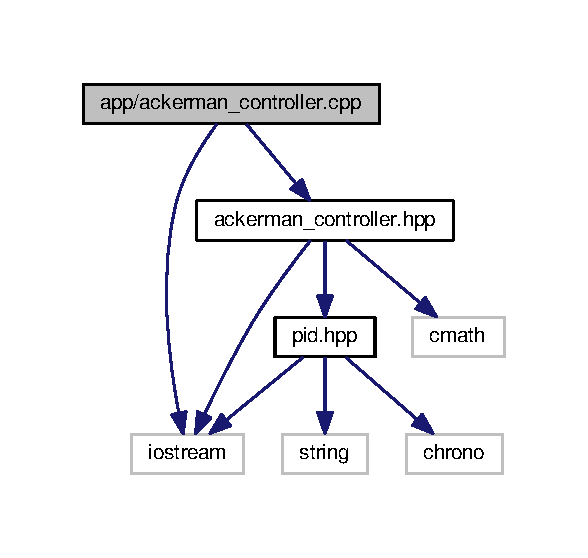
\includegraphics[width=282pt]{ackerman__controller_8cpp__incl}
\end{center}
\end{figure}


\subsection{Detailed Description}
Defines the function to calculate the Radius, wheel velocity and update the current heading.  \char`\"{}\+Copyright 2019 $<$\+Ashwin Varghese Kuruttukulam$>$
@\+Copyright \char`\"{}Copyright 2019 $<$\+Charan karthikeyan$>$=\char`\"{}\char`\"{}$>$ 

\begin{DoxyAuthor}{Author}
Ashwin Varghese Kuruttukulam 

Charan Karthikeyan 
\end{DoxyAuthor}

\hypertarget{ackerman__sim_8cpp}{}\section{app/ackerman\+\_\+sim.cpp File Reference}
\label{ackerman__sim_8cpp}\index{app/ackerman\+\_\+sim.\+cpp@{app/ackerman\+\_\+sim.\+cpp}}


Declarations of the function to simulate the ackerman steering  \char`\"{}\+Copyright 2019 $<$\+Ashwin Varghese Kuruttukulam$>$
@\+Copyright \char`\"{}Copyright 2019 $<$\+Charan karthikeyan$>$=\char`\"{}\char`\"{}$>$  


{\ttfamily \#include \char`\"{}ackerman\+\_\+sim.\+hpp\char`\"{}}\\*
Include dependency graph for ackerman\+\_\+sim.\+cpp\+:
\nopagebreak
\begin{figure}[H]
\begin{center}
\leavevmode
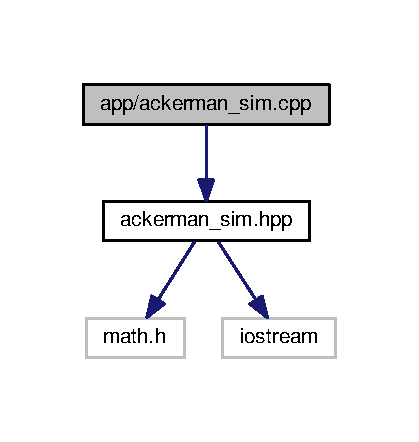
\includegraphics[width=201pt]{ackerman__sim_8cpp__incl}
\end{center}
\end{figure}


\subsection{Detailed Description}
Declarations of the function to simulate the ackerman steering  \char`\"{}\+Copyright 2019 $<$\+Ashwin Varghese Kuruttukulam$>$
@\+Copyright \char`\"{}Copyright 2019 $<$\+Charan karthikeyan$>$=\char`\"{}\char`\"{}$>$ 

\begin{DoxyAuthor}{Author}
Ashwin Varghese Kuruttukulam 

Charan Karthikeyan 
\end{DoxyAuthor}

\hypertarget{main_8cpp}{}\section{app/main.cpp File Reference}
\label{main_8cpp}\index{app/main.\+cpp@{app/main.\+cpp}}


Main program that runs the pid, ackerman controller and the ackerman simulation classes.  


{\ttfamily \#include $<$iostream$>$}\\*
{\ttfamily \#include \char`\"{}ackerman\+\_\+controller.\+hpp\char`\"{}}\\*
{\ttfamily \#include \char`\"{}ackerman\+\_\+sim.\+hpp\char`\"{}}\\*
Include dependency graph for main.\+cpp\+:
\nopagebreak
\begin{figure}[H]
\begin{center}
\leavevmode
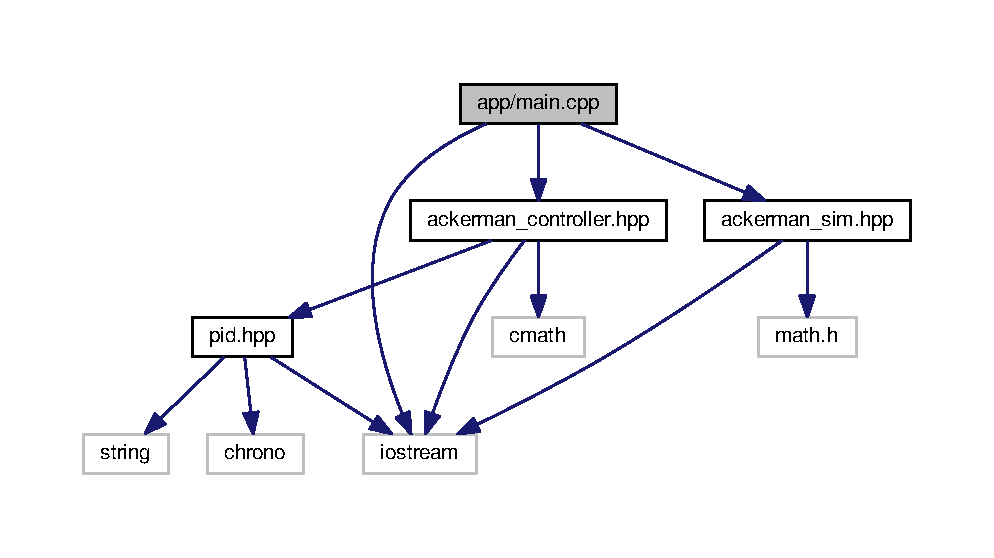
\includegraphics[width=350pt]{main_8cpp__incl}
\end{center}
\end{figure}
\subsection*{Functions}
\begin{DoxyCompactItemize}
\item 
int {\bfseries main} ()\hypertarget{main_8cpp_ae66f6b31b5ad750f1fe042a706a4e3d4}{}\label{main_8cpp_ae66f6b31b5ad750f1fe042a706a4e3d4}

\end{DoxyCompactItemize}


\subsection{Detailed Description}
Main program that runs the pid, ackerman controller and the ackerman simulation classes. 

\begin{DoxyAuthor}{Author}
Ashwin Varghese Kuruttukulam 

Charan Karthikeyan  \char`\"{}\+Copyright 2019 $<$\+Ashwin Varghese Kuruttukulam$>$
@\+Copyright \char`\"{}Copyright 2019 $<$\+Charan karthikeyan$>$=\char`\"{}\char`\"{}$>$ 
\end{DoxyAuthor}

\hypertarget{pid_8cpp}{}\section{app/pid.cpp File Reference}
\label{pid_8cpp}\index{app/pid.\+cpp@{app/pid.\+cpp}}


Definition of the P\+ID class to calculate the feedback  \char`\"{}\+Copyright 2019 $<$\+Ashwin Varghese Kuruttukulam$>$
@\+Copyright \char`\"{}Copyright 2019 $<$\+Charan karthikeyan$>$=\char`\"{}\char`\"{}$>$  


{\ttfamily \#include \char`\"{}pid.\+hpp\char`\"{}}\\*
{\ttfamily \#include $<$chrono$>$}\\*
Include dependency graph for pid.\+cpp\+:
\nopagebreak
\begin{figure}[H]
\begin{center}
\leavevmode
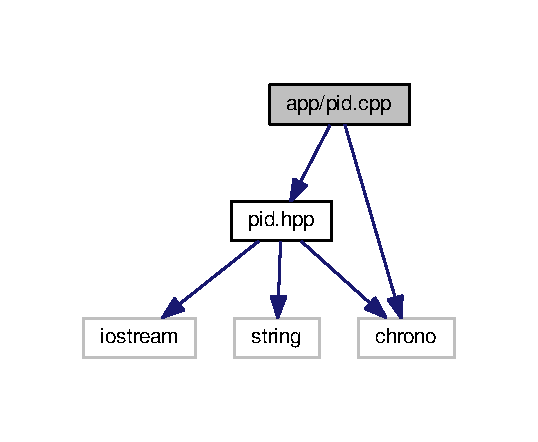
\includegraphics[width=258pt]{pid_8cpp__incl}
\end{center}
\end{figure}


\subsection{Detailed Description}
Definition of the P\+ID class to calculate the feedback  \char`\"{}\+Copyright 2019 $<$\+Ashwin Varghese Kuruttukulam$>$
@\+Copyright \char`\"{}Copyright 2019 $<$\+Charan karthikeyan$>$=\char`\"{}\char`\"{}$>$ 

\begin{DoxyAuthor}{Author}
Ashwin Varghese Kuruttukulam 

Charan Karthikeyan 
\end{DoxyAuthor}

\hypertarget{ackerman__sim_8hpp}{}\section{include/ackerman\+\_\+sim.hpp File Reference}
\label{ackerman__sim_8hpp}\index{include/ackerman\+\_\+sim.\+hpp@{include/ackerman\+\_\+sim.\+hpp}}


Defines the function to simulate the ackerman steering  \char`\"{}\+Copyright 2019 $<$\+Ashwin Varghese Kuruttukulam$>$
@\+Copyright \char`\"{}Copyright 2019 $<$\+Charan karthikeyan$>$=\char`\"{}\char`\"{}$>$  


{\ttfamily \#include $<$math.\+h$>$}\\*
{\ttfamily \#include $<$iostream$>$}\\*
Include dependency graph for ackerman\+\_\+sim.\+hpp\+:
\nopagebreak
\begin{figure}[H]
\begin{center}
\leavevmode
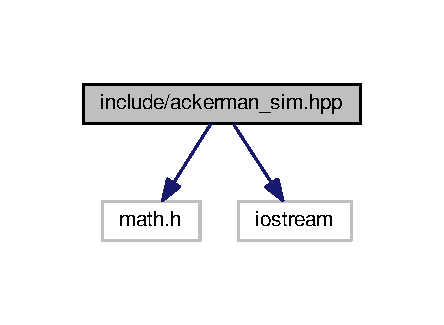
\includegraphics[width=213pt]{ackerman__sim_8hpp__incl}
\end{center}
\end{figure}
This graph shows which files directly or indirectly include this file\+:
\nopagebreak
\begin{figure}[H]
\begin{center}
\leavevmode
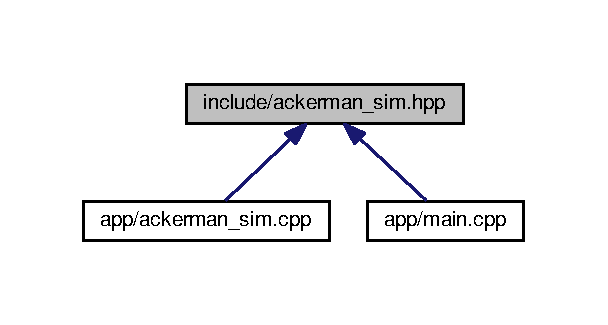
\includegraphics[width=292pt]{ackerman__sim_8hpp__dep__incl}
\end{center}
\end{figure}
\subsection*{Classes}
\begin{DoxyCompactItemize}
\item 
class \hyperlink{classackerman__sim}{ackerman\+\_\+sim}
\end{DoxyCompactItemize}


\subsection{Detailed Description}
Defines the function to simulate the ackerman steering  \char`\"{}\+Copyright 2019 $<$\+Ashwin Varghese Kuruttukulam$>$
@\+Copyright \char`\"{}Copyright 2019 $<$\+Charan karthikeyan$>$=\char`\"{}\char`\"{}$>$ 

\begin{DoxyAuthor}{Author}
Ashwin Varghese Kuruttukulam 

Charan Karthikeyan 
\end{DoxyAuthor}

\hypertarget{pid_8hpp}{}\section{include/pid.hpp File Reference}
\label{pid_8hpp}\index{include/pid.\+hpp@{include/pid.\+hpp}}


Defines a P\+ID Controller from the feedback/measured value and the setpoint. The output of the P\+ID is calculated as per the equation output = Kp$\ast$\+Error + Ki$\ast$\+Error\+Sum$\ast$dt + Kp$\ast$(Error-\/prev\+Error)/dt.  


{\ttfamily \#include $<$iostream$>$}\\*
{\ttfamily \#include $<$string$>$}\\*
{\ttfamily \#include $<$chrono$>$}\\*
Include dependency graph for pid.\+hpp\+:
\nopagebreak
\begin{figure}[H]
\begin{center}
\leavevmode
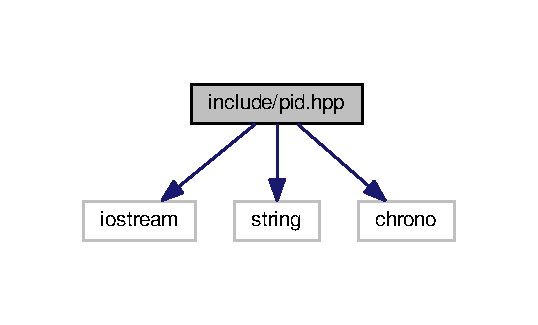
\includegraphics[width=258pt]{pid_8hpp__incl}
\end{center}
\end{figure}
This graph shows which files directly or indirectly include this file\+:
\nopagebreak
\begin{figure}[H]
\begin{center}
\leavevmode
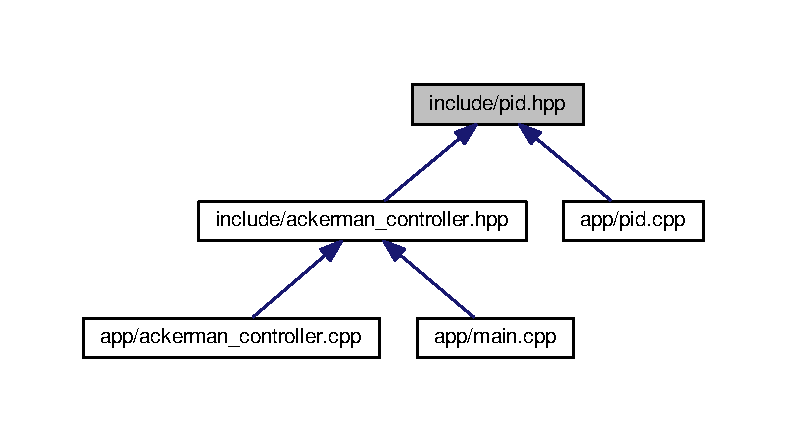
\includegraphics[width=350pt]{pid_8hpp__dep__incl}
\end{center}
\end{figure}
\subsection*{Classes}
\begin{DoxyCompactItemize}
\item 
class \hyperlink{classpid}{pid}
\end{DoxyCompactItemize}


\subsection{Detailed Description}
Defines a P\+ID Controller from the feedback/measured value and the setpoint. The output of the P\+ID is calculated as per the equation output = Kp$\ast$\+Error + Ki$\ast$\+Error\+Sum$\ast$dt + Kp$\ast$(Error-\/prev\+Error)/dt. 

\begin{DoxyAuthor}{Author}
Ashwin Varghese Kuruttukulam 

Charan Karthikeyan  \char`\"{}\+Copyright 2019 $<$\+Ashwin Vargheese Kuruttukulam$>$
@\+Copyright \char`\"{}Copyright 2019 $<$\+Charan karthikeyan$>$=\char`\"{}\char`\"{}$>$ 
\end{DoxyAuthor}

%--- End generated contents ---

% Index
\backmatter
\newpage
\phantomsection
\clearemptydoublepage
\addcontentsline{toc}{chapter}{Index}
\printindex

\end{document}
